\newsection{Segnalazione errori}
Nel caso in cui dovessero essere riscontrati eventuali errori o criticità è possibile segnalarli attraverso l'indirizzo email del gruppo oppure aprendo una segnalazione nell'apposita sezione \gl{issue} della \gl{repository} in cui risiede il plugin.

\subsection{Segnalazione per email}
L'indirizzo del gruppo è: {\url{7dos.swe@gmail.com}}. \\
Inserire nell'oggetto la segnatura [BUG] per segnalare che si tratta di un errore, seguita da una breve e concisa descrizione dello stesso.
Indicare nel corpo dell'email la versione di Grafana usata, la versione del plugin ed una descrizione dettagliata dell'errore riscontrato.

\begin{figure} [H]
	\centering
	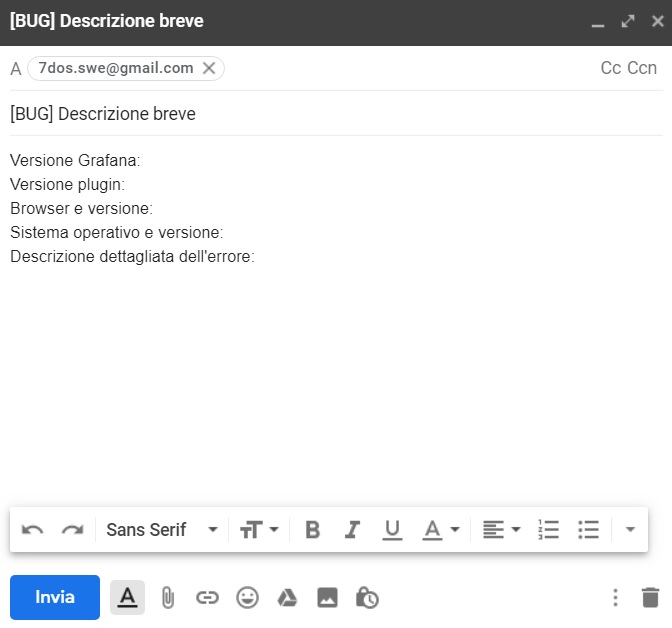
\includegraphics[scale=0.9]{Img/email.jpg} 
	\caption{Template email} \label{} 
\end{figure} 

\subsection{Segnalazione con issue}
La root del plugin è: \url{https://github.com/NicoloTartaggia/7DOS-plugin}. \\
Posizionarsi nella sezione \emph{"Issues"} e premere il pulsante \emph{"New issue"}. Inserire nel titolo la segnatura [BUG] per segnalare che si tratta di un errore, seguita da una breve e concisa descrizione dello stesso.
Indicare nel corpo della issue la versione di Grafana usata, la versione del plugin ed una descrizione dettagliata dell'errore riscontrato.
\begin{figure} [H]
	\centering
	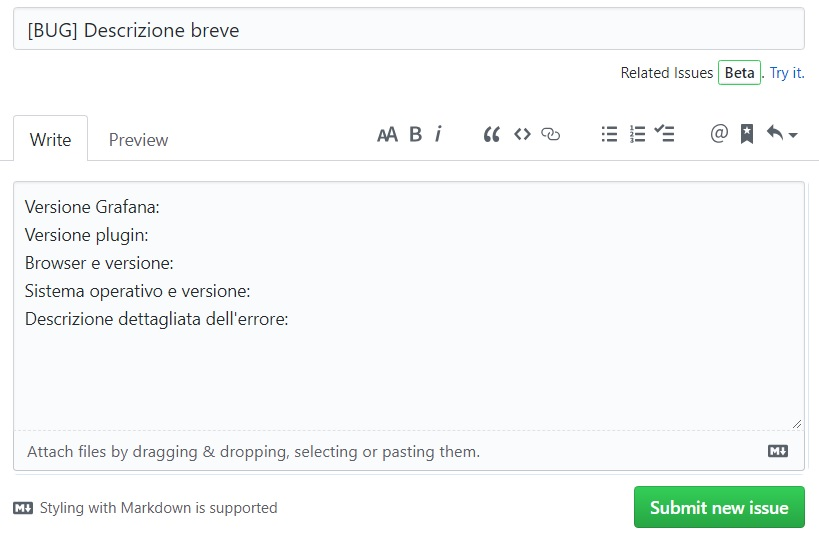
\includegraphics[scale=0.9]{Img/issue.jpg} 
	\caption{Template issue} \label{} 
\end{figure} 

\newpage